\documentclass[aspectratio=43]{beamer}
\usepackage[latin1]{inputenc}
\usepackage{amsmath}
\usepackage{amsfonts}
\usepackage{amssymb}
\usepackage{makeidx}
\usepackage{graphicx}
\usepackage{array}

% Customization
\mode<presentation>{
\usetheme{CambridgeUS}
\usecolortheme{dolphin}
\setbeamertemplate{navigation symbols}{}
}

%\setbeamertemplate{footline}[frame number]

%TikZ diagrams
\usepackage{tikz}
\usetikzlibrary{patterns}
\usetikzlibrary{arrows,shapes}
\usetikzlibrary{shapes.multipart}
\usetikzlibrary{trees}
\usetikzlibrary{shapes.geometric}
\usetikzlibrary{matrix,arrows}
\usetikzlibrary{positioning}
\usetikzlibrary{calc,through}
\usetikzlibrary{decorations.pathreplacing}
\usepackage{pgffor}

% Define colors
\definecolor{darkgreen}{rgb}{0.0, 0.5, 0.13}
\definecolor{darkblue}{rgb}{0.0, 0.0, 0.55}
\definecolor{darkred}{rgb}{0.55, 0.0, 0.0}

% For using TikZ
\usetikzlibrary{decorations.pathmorphing}
\usetikzlibrary{decorations.markings}
\tikzset{
	vector/.style={decorate, decoration={snake,amplitude=3pt}, draw},
	gluon/.style={decorate, decoration={coil,amplitude=2.5pt},draw},
	provector/.style={decorate, decoration={snake,amplitude=2.5pt}, draw},
	antivector/.style={decorate, decoration={snake,amplitude=-2.5pt}, draw},
	fermion/.style={draw=black, postaction={decorate},
		decoration={markings,mark=at position .55 with {\arrow[draw=black,thick]{>}}}},
	fermionbar/.style={draw=black, postaction={decorate},
		decoration={markings,mark=at position .55 with {\arrow[draw=black,thick]{<}}}},
	fermionnoarrow/.style={draw=black},
	gluon/.style={decorate, draw=black,
		decoration={coil,amplitude=2.5pt, segment length=3pt}},
	gluon2/.style={decorate, draw=black,
		decoration={coil,amplitude=1.75pt, segment length=2.75pt}},
	scalar/.style={dashed,draw=black, postaction={decorate},
		decoration={markings,mark=at position .55 with {\arrow[draw=black]{>}}}},
	scalarbar/.style={dashed,draw=black, postaction={decorate},
		decoration={markings,mark=at position .55 with {\arrow[draw=black]{<}}}},
	scalarnoarrow/.style={dashed,draw=black},
	electron/.style={draw=black, postaction={decorate},
		decoration={markings,mark=at position .55 with {\arrow[draw=black]{>}}}},
	bigvector/.style={decorate, decoration={snake,amplitude=4pt}, draw},
}

% Blocks
\tikzstyle{block} = [draw, rectangle, minimum height = 3em, rounded corners, minimum width = 4em]
\tikzstyle{block2} = [draw, rectangle, minimum height = 3em, rounded corners, minimum width = 7em]
\tikzstyle{circle} = [draw, circle, radius = 1.5]
\tikzstyle{arrow} = [thick,->]
%************************************************************************************************************

% Title and author
\title[QCD and Monte Carlo]{QCD and Monte Carlo}
\author{\textbf {Jes\'us Urtasun Elizari}}
%\institute{\textbf {University of Milan}}
\date{Milan, September 2020}

\begin{document}

% Front slide
\begin{frame}

	%\maketitle
	\vspace{1.0 cm}
	
	\center{\color{blue}Perturbative QCD and Monte Carlo event generators}
	
	\vspace{0.25 cm}
	\center{Monte Carlo course seminar - Milan, September 2020}

	\begin{figure}
		\minipage{1\textwidth}
		
\includegraphics[width = 3.0 cm]{plots/logo_unimi.png}
		\hfill
		
\includegraphics[width = 3.0 cm]{plots/logo_infn.png}
		\hfill
		
\includegraphics[width = 3.0 cm]{plots/logo_erc.png}
		\endminipage
	\end{figure}

	\vspace{1.0 cm}

\end{frame}

% Introduction
\begin{frame}

	\frametitle{Outline}
	
	\begin{enumerate}
		\item {\color{blue}Hadron collisions}
		\begin{itemize}
			\item Hadron collisions and strong interactions
			\item Renormalization group
			\item Jets and IR divergences
		\end{itemize}
		\item {\color{blue}Collinear factorization}
		\begin{itemize}
			\item Factorization theorem
			\item Kinematics of splitting
			\item Recursive factorization
		\end{itemize}
		\item {\color{blue}Parton showers}
		\begin{itemize}
			\item Final state radiation
			\item Initial state radiation
			\item Ordering variables (PYTHIA and HERWIG)
		\end{itemize}
	\end{enumerate}
	
\end{frame}

% Hadron collisions
\begin{frame}

\center{\color{blue}Hadron collisions}

\end{frame}

% Hadron collisions I
\begin{frame}

	\frametitle{Hadron collisions}
	\framesubtitle{QCD from $e^{+}e^{-}$ annihilation}

	\begin{figure}
		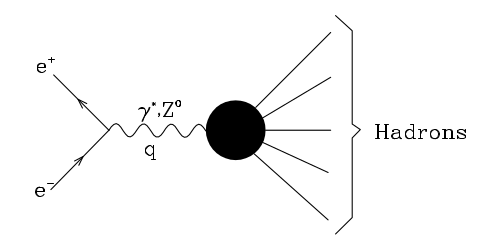
\includegraphics[width = 5 cm]{plots/ee_hadrons.png}
	\end{figure}
 
	QCD arise already from $e^{+}e^{-}$ annihilation $\rightarrow R_{0}$ ratio
	\begin{figure}
		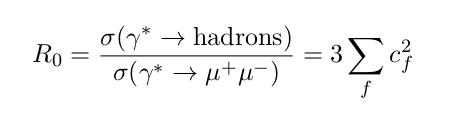
\includegraphics[width = 6 cm]{plots/eq_R0.png}
	\end{figure}

	\begin{enumerate}
		\item Color factor (3 color for each quark)
		\item Sum over charges of different flavour quarks
		\item Corrections near the threshold and at higher orders

	\end{enumerate}	
	
\end{frame}

% Hadron collisions II
\begin{frame}

	\frametitle{Hadron collisions}
	\framesubtitle{QCD from $e^{+}e^{-}$ annihilation}
	
	\begin{figure}
		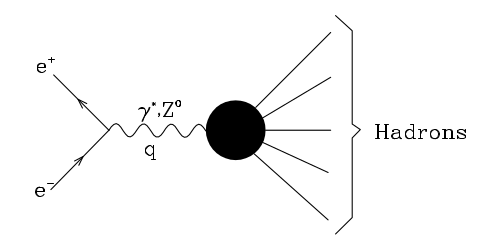
\includegraphics[width = 5 cm]{plots/ee_hadrons.png}
	\end{figure}	
	
	Consider corrections to $R_{0}$ from gluon radiation. Renormalize coupling.
	\begin{figure}
		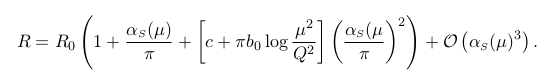
\includegraphics[width = 10 cm]{plots/eq_R0_3.png}
	\end{figure}

	Define renormalized coupling, running with the scale \\
	UV logarithmic divergence in $\log(\mu^{2} / Q^{2})$
\end{frame}

% Hadron collisions III
\begin{frame}
	
	\frametitle{Hadron collisions}
	\framesubtitle{QCD from $e^{+}e^{-}$ annihilation}
	
	Questions for a field theory
	\begin{enumerate}
		\item Can we go to arbitrarily large energies? $\rightarrow$ divergences arise, renormalization / factorization needed
		\item Can we compute $R_{0}$ for every process? $\rightarrow$ IR observables
	\end{enumerate}	

\end{frame}

% Renormalization group I
\begin{frame}

	\frametitle{Hadron collisions}
	\framesubtitle{Renormalization group}
	
	\begin{itemize}
		\item UV divergences are encountered in field theories
		\item Take a physical quantity $G$ depending on a scale $M$, a coupling $\alpha$ and some invariants $s_{1}, ..., s_{n}$	
		\item Define a "renormalized" coupling $\alpha_{\textrm{Ren}} = \alpha + c_{1}\alpha^{2} + c_{2}\alpha^{3} + ...$
	\end{itemize}
 
	The physical quantity in terms of $\{\alpha, M\}$ and $\{\alpha_{\textrm{Ren}}, \mu\}$ 
	\begin{figure}
		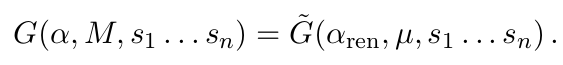
\includegraphics[width = 7 cm]{plots/eq_RGE.png}
	\end{figure}

	{\color{blue}Physics must be invariant under change of $\{\alpha_{\textrm{Ren}}, \mu\}$}
	\begin{figure}
		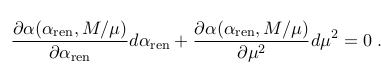
\includegraphics[width = 7 cm]{plots/eq_RGE_2.png}
	\end{figure}

\end{frame}

% Renormalization group II
\begin{frame}

	\frametitle{Hadron collisions}
	\framesubtitle{Renormalization group}
	
	\begin{itemize}
		\item Running coupling given by Renormalization Group Equation (RGE)
		\begin{equation}
		{\color{blue}\mu\frac{d\alpha_{s}(\mu)}{d\mu} = \beta(\alpha_{s}(\mu)) = -\sum_{n = 0}^{\infty} \beta_{n} \Big( \frac{\alpha_{s}}{\pi} \Big)^{n + 1}} \nonumber
		\end{equation}
		\item Coupling {\color{blue}$\alpha_{s}$} evolves with scale {\color{blue}$\mu$} as given by RGE $\rightarrow$ LO behavior driven by $\beta_{0}$
		\item $\beta_{0}^{\textrm{QCD}} > 0 \implies$ weakly coupled at large energies, asymptotic freedom
		\item $\beta_{0}^{\textrm{QED}} < 0 \implies$ strongly coupled at large energies, UV divergent!
		
	\end{itemize}

\end{frame}

% Jets in e+e- I
\begin{frame}
	
	\frametitle{Hadron collisions}
	\framesubtitle{Jets in $e^{+}e^{-}$}
	
	Consider $\alpha_{s}$ corrections to born level amplitude
	
	\begin{figure}
		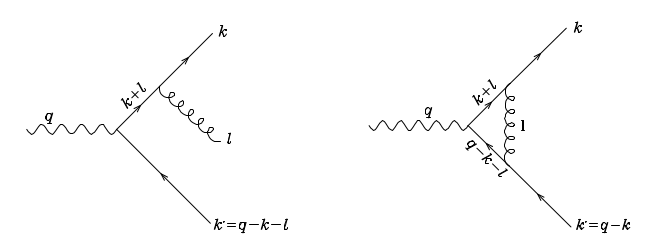
\includegraphics[width = 7 cm]{plots/qcd_corrections_2.png}
	\end{figure}

	\begin{align}
		\mathcal{M}_{\textrm{Born}} &= \bar{u}(k)\epsilon^{\mu}\gamma_{\mu}v(k') \nonumber \\
		\mathcal{M}_{1} &= \mathcal{M} \frac{k_{\alpha}}{k \cdot l} \longrightarrow \textrm{Real radiation} \nonumber \\
		\mathcal{M}_{1} &= -\mathcal{M} \frac{k'_{\alpha}}{k' \cdot l} \longrightarrow \textrm{Virtual contribution} \nonumber		 
	\end{align}

\end{frame}

% Jets in e+e- II
\begin{frame}

	\frametitle{Hadron collisions}
	\framesubtitle{Jets in $e^{+}e^{-}$}
	
	Consider $\alpha_{s}$ corrections to born level amplitude
	
	\begin{figure}
		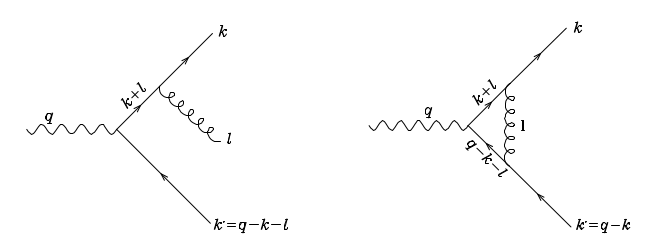
\includegraphics[width = 7 cm]{plots/qcd_corrections_2.png}
	\end{figure}
	
	Sum real and virtual contributions to the Born matrix element, square and integrate with phase space element $d^{3}l = (l^{0})^{2} dl^{0} d\cos\theta d\phi$
	\begin{figure}
		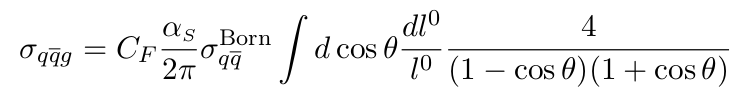
\includegraphics[width = 9.5 cm]{plots/eq_qqbg.png}
	\end{figure}

\end{frame}

% Jets in e+e- III
\begin{frame}

	\frametitle{Hadron collisions}
	\framesubtitle{Jets in $e^{+}e^{-}$}
	
	\begin{figure}
		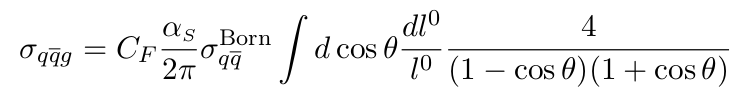
\includegraphics[width = 9.5 cm]{plots/eq_qqbg.png}
	\end{figure}

	\begin{itemize}
		\item Soft $(l^{0} \rightarrow 0)$ and collinear $(\theta \rightarrow 0, \pi)$ divergences
		\item No renormalization procedure to apply $\rightarrow$ divergences coming from long distance effects (fermion masses, hadronization, etc)
		\item Kinoshita-Lee-Nauemberg theorem {\color{blue}(*)}
	\end{itemize}

	{\color{blue}Understand Born cross section as the LO term in a well defined perturbative expansion}
	
\end{frame}

% Jets in e+e- IV
\begin{frame}

	\frametitle{Hadron collisions}
	\framesubtitle{Sterman-Weinberg jets}
	
	Sterman - Weinberg jets. "In a hadronic event with CM energy $E$, 2 cones can be found with opening $\delta$ containing $(1 - \epsilon)$ fraction of $E$."
	
	\begin{figure}
		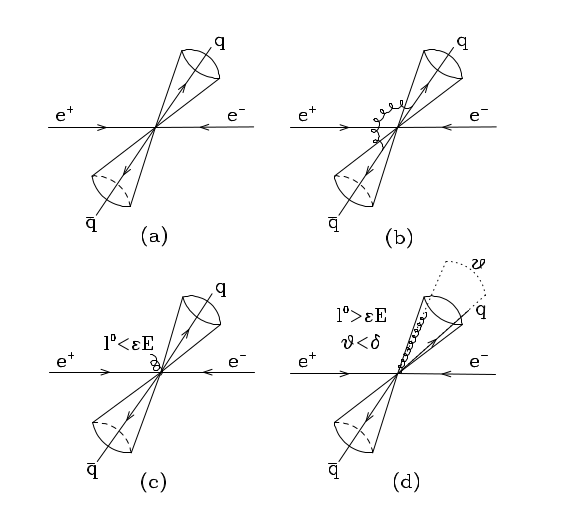
\includegraphics[width = 7 cm]{plots/SW_jets.png}
	\end{figure}

\end{frame}

% Jets in e+e- V
\begin{frame}

	\frametitle{Hadron collisions}
	\framesubtitle{Sterman-Weinberg jets}
	
	Sterman - Weinberg jets. "In a hadronic event with CM energy $E$, 2 cones can be found with opening $\delta$ containing $(1 - \epsilon)$ fraction of $E$."
	
	\begin{figure}
		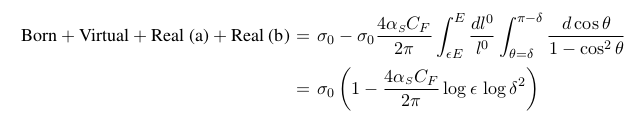
\includegraphics[width = 12 cm]{plots/eq_SW_jets.png}
	\end{figure}

	When all contributions summed, the cross section is no longer singular {\color{red}(*)} \\
	Computed in terms of partons, but representing hadronic final state \\
	Jets as IR finite final state {\color{red}(*)}
	
\end{frame}

% Collinear factorization
\begin{frame}

	\center{\color{blue}Collinear factorization}

\end{frame}

% Collinear factorization I
\begin{frame}

	\frametitle{Collinear factorization}
	\framesubtitle{QCD from $e^{+}e^{-}$ annihilation}
	
	\begin{itemize} 
		\item When computing partonic cross section, collinear partons can be emitted from incoming/outgoing parton
		\item $\sigma$ dominated by collinear decay of parton with small virtuality
	\end{itemize}

	\begin{figure}
		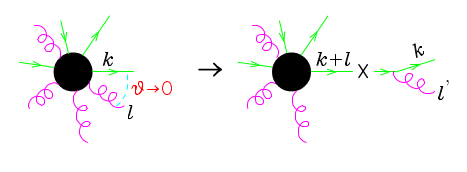
\includegraphics[width = 7 cm]{plots/collinear_factorization.png}
	\end{figure}

	Factorization theorem $\longrightarrow$ Factor out tree level amplitude and splitting
	\begin{figure}
	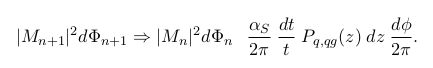
\includegraphics[width = 8 cm]{plots/eq_factorization_theorem.png}
	\end{figure}
	
\end{frame}

% Collinear factorization II
\begin{frame}

	\frametitle{Collinear factorization}
	\framesubtitle{QCD from $e^{+}e^{-}$ annihilation}
	
	\begin{itemize} 
		\item Kinematics of splitting $(t, z, \phi)$
		\begin{itemize}
			\item $t$ has dimensions of energy (virtuality, $p_{\perp}$, angular variable)
			\item $z$ represents the fraction of momentum of radiated parton
			\item $\phi$ represents azimuth of the $k, l$ plane
		\end{itemize}
	
	\vspace{0.5cm}
	
		\item Factorization holds for small angles. Applied recursively
	\end{itemize}
	
	\begin{figure}
		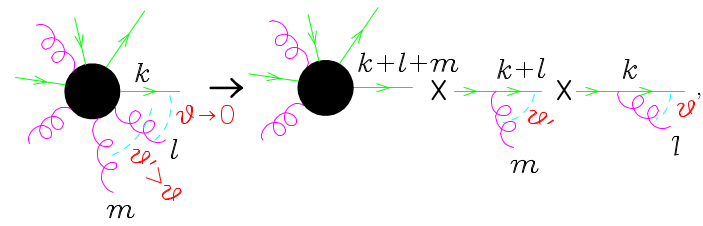
\includegraphics[width = 7 cm]{plots/shower_4.png}
	\end{figure}

\end{frame}

% Parton showers
\begin{frame}

	\center{\color{blue}Parton showers and MC generators}

\end{frame}

% Shower equation I
\begin{frame}

	\frametitle{Parton showers and MC generators}
	\framesubtitle{Formal representation of a shower}
	
	Approximated description of a hadronic final state. Model a given hard scattering with arbitrary number of enhanced radiations
	
	\begin{figure}
		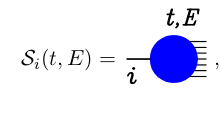
\includegraphics[width = 4 cm]{plots/shower_1.png}
	\end{figure}
		
	\begin{itemize} 
		\item Enseble of all possible showers from a parton {\color{blue}i} at scale {\color{blue}t}
		\item Sudakov form factor $\Delta_{i}(t, t_{0})$  such that $\Delta_{i}(t_{0}, t_{0})$ = 1
		\item Shower $S_{i}(t, E)$ 	such that $S_{i}^{\textrm{inc}} = \sum_{\mathcal{F}} S_{i}(t, E) = 1 $
	\end{itemize}

\end{frame}

% Shower equation II
\begin{frame}

	\frametitle{Parton showers and MC generators}
	\framesubtitle{Formal representation of a shower}
	 
	 
	 Ensemble of all possible radiations as the sum of no radiation, with radiation and shower from radiated partons
	\begin{figure}
		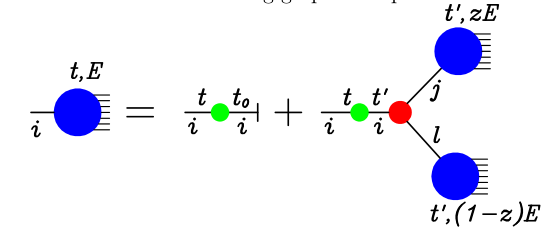
\includegraphics[width = 7 cm]{plots/shower_2.png}
	\end{figure}
	
	\begin{itemize} 
		\item Ansatz for Sudakov $$\Delta_{i}(t, t') = \exp\Bigg\{- \int_{t'}^{t} \frac{dt''}{t''}\int dz \sum_{jl} P_{i, jl}(z) \frac{\alpha_{s}(t')}{2\pi} \Bigg\}$$
		\item Therefore $\partial \Delta(t, t') / \partial t \propto \Delta(t, t') \longrightarrow$ apply shower recursively
	\end{itemize}

\end{frame}

% Shower equation III
\begin{frame}

	\frametitle{Parton showers and MC generators}
	\framesubtitle{Shower algorithm}
	
	Generate hard process with probability proportional to its parton level cross section. For each final state colored parton:
	\begin{enumerate} 
		\item Set scale $t$ to $Q$, hard scale of the process
		\item Generate random number $0 < r < 1$
		\item Solve $r = \Delta_{i}(t, t')$ for t'
		\item i) if $t' < t_{0}$, no further branching and stop shower
		\item ii) if $t' \geq t_{0}$, one branching into partons $j, l$ with energies $E_{j} = zE_{i}$ and $E_{l} = (1 - z)E_{i}$, z following the $P_{i, jl}(z)$ distribution and $\phi$ uniform in the interval $[0, 2\pi]$
		\item For each branched partons set $t = t'$ and start from (2)
	\end{enumerate}

\end{frame}

% Shower equation ISR I
\begin{frame}

	\frametitle{Parton showers and MC generators}
	\framesubtitle{Initial state radiation}
	
	ISR already important in QED $\longrightarrow$ Used to determine the $Z$ peak at LEP
	\begin{figure}
		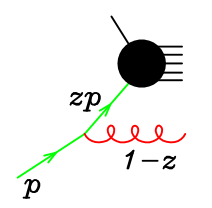
\includegraphics[width = 3 cm]{plots/shower_ISR.png}
	\end{figure}
	
	\begin{itemize}
		\item QCD coupling much larger $\longrightarrow$ QCD ISR even more important
		\item Specially large for small momentum transfer
		\item Same as final state partons \textit{always} manifest as jets, initial state ones \textit{always} lead to ISR
	\end{itemize}
	
\end{frame}

% Shower equation ISR II
\begin{frame}

	\frametitle{Parton showers and MC generators}
	\framesubtitle{Initial state radiation}
	
	\begin{figure}
		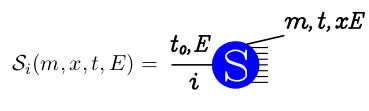
\includegraphics[width = 5.5 cm]{plots/shower_ISR_2.png}
	\end{figure}
	
	\begin{itemize} 
		\item Lines between $t_{1}$ and $t_{2}$ (consecutive radiations) are spacelike {\color{blue}(*)}
		\item Difference in Sudakov factors and Splitting functions start at NLO
	\end{itemize}
	
	\begin{figure}
		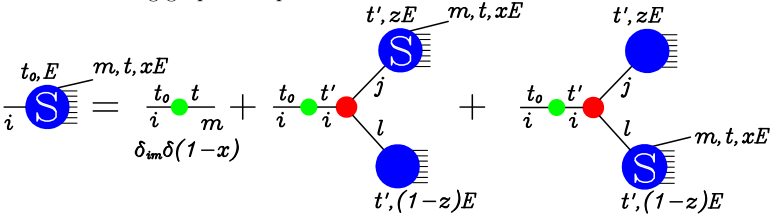
\includegraphics[width = 10 cm]{plots/shower_ISR_3.png}
	\end{figure}

\end{frame}

% Shower equation III
\begin{frame}

	\frametitle{Parton showers and MC generators}
	\framesubtitle{Ordering variables}
	
	HERWIG
	\begin{itemize} 
		\item Ordering variable $t = E^{2}\theta^{2}/2$
		\item Order of transverse momentum as "angular ordering"
		\item IR cut-off needed
	\end{itemize}

	PYTHIA
	\begin{itemize} 
		\item There is not angular ordering
		\item More natural kinematics
		\item Unphysical increase of number of partons $\longrightarrow$ solve by imposing veto to branchings that violate angular ordering
	\end{itemize}

\end{frame}

\end{document}